\documentclass[10pt, a4paper, landscape]{article}

% ----- packages -----
\usepackage{amsmath} % AMS mathematical facilities for LaTeX
\usepackage{amssymb}
\usepackage{enumitem} % Control layout of itemize, enumerate, description
\usepackage{fancyhdr} % Extensive control of page headers and footers in LaTeX2
\usepackage{geometry} % Flexible and complete interface to document dimensions
\usepackage{graphicx} % Enhanced support for graphics
\usepackage{hyperref} % Extensive support for hypertext in LaTeX
\usepackage{multicol} % Intermix single and multiple columns
\usepackage{parskip} % Layout with zero \parindent, non-zero \parskip
\usepackage{tikz} % Create PostScript and PDF graphics in TeX
\usepackage{titlesec} % Select alternative section titles

% ----- random seed -----
\pgfmathsetseed{10}

% ----- custom commands -----
\newcommand{\E}{\mathrm{E}}
\newcommand{\Var}{\mathrm{Var}}
\newcommand{\se}{\mathrm{ee}}
\newcommand{\Cov}{\mathrm{Cov}}
\newcommand{\Corr}{\mathrm{Corr}}
\newcommand{\SSR}{\mathrm{SRC}}
\newcommand{\SSE}{\mathrm{SEC}}
\newcommand{\SST}{\mathrm{STC}}
\newcommand{\tr}{\mathsf{T}}
\newcommand{\rk}{\mathrm{rg}}

% ----- page customization -----
\geometry{margin=1cm} % margins config
\pagenumbering{gobble} % remove page numeration
\setlength{\parskip}{0cm} % paragraph spacing
% title spacing
\titlespacing{\section}{0pt}{2ex}{1ex}
\titlespacing{\subsection}{0pt}{1ex}{0ex}
\titlespacing{\subsubsection}{0pt}{0.5ex}{0ex}

% ----- footer -----
\pagestyle{fancy}
\renewcommand{\headrulewidth}{0pt}
\cfoot{\href{https://github.com/marcelomijas/econometrics-cheatsheet}{\normalfont \footnotesize ADD-24.6-ES - github.com/marcelomijas/econometrics-cheatsheet - Licencia CC-BY-4.0}}
\setlength{\footskip}{12pt}

% ----- document -----
\begin{document}
	\begin{multicols}{3}
		\begin{center}
			\textbf{\LARGE \href{https://github.com/marcelomijas/econometrics-cheatsheet}{Cheat Sheet Adicional}}
			
			{\footnotesize Por Marcelo Moreno - Universidad Rey Juan Carlos}
			
			{\footnotesize The Econometrics Cheat Sheet Project}
		\end{center}
		
		\section*{Notación matricial MCO}
		
		El modelo econométrico general:
		
		\begin{center}
			$y_{i} = \beta_{0} + \beta_{1} x_{1i} + \cdots + \beta_{k} x_{ki} + u_{i}$
		\end{center}
		
		Puede ser escrito en notación matricial como:
		
		\begin{center}
			$y = X \beta + u$
		\end{center}
		
		Llamemos $\hat{u}$ al vector de residuos estimados ($\hat{u} \neq u$):
		
		\begin{center}
			$\hat{u} = y - X \hat{\beta}$
		\end{center}
		
		El \textbf{objetivo} de MCO es \textbf{minimizar} la SRC:
		
		\begin{center}
			$\min \SSR = \min \sum_{i=1}^{n} \hat{u}_{i}^{2} = \min \hat{u}^{\tr} \hat{u}$
		\end{center}
		
		\begin{itemize}[leftmargin=*]
			\item Definiendo $\hat{u}^{\tr} \hat{u}$:
			
			\begin{center}
				$\hat{u}^{\tr} \hat{u} = (y - X \hat{\beta})^{\tr} (y - X \hat{\beta}) =$
				
				$= y^{\tr} y - 2 \hat{\beta}^{\tr} X^{\tr} y + \hat{\beta}^{\tr} X^{\tr} X \hat{\beta}$
			\end{center}
			
			\item Minimizando $\hat{u}^{\tr} \hat{u}$:
			
			\begin{center}
				$\frac{\partial \hat{u}^{\tr} \hat{u}}{\partial \hat{\beta}} = -2 X^{\tr} y + 2 X^{\tr} X \hat{\beta} = 0$
				
				$\hat{\beta} = (X^{\tr} X)^{-1} (X^{\tr} y)$
				
				\scalebox{0.85}{
					$
					\begin{bmatrix}
						\beta_{0} \\
						\beta_{1} \\
						\vdots    \\
						\beta_{k}
					\end{bmatrix}
					=
					\begin{bmatrix}
						n          & \sum x_{1}       & \hdots & \sum x_{k}       \\
						\sum x_{1} & \sum x_{1}^{2}   & \hdots & \sum x_{1} x_{k} \\
						\vdots     & \vdots           & \ddots & \vdots           \\
						\sum x_{k} & \sum x_{k} x_{1} & \hdots & \sum x_{k}^{2}
					\end{bmatrix}^{-1}\cdot
					\begin{bmatrix}
						\sum y       \\
						\sum y x_{1} \\
						\vdots       \\
						\sum y x_{k}
					\end{bmatrix}
					$ 
				}
			\end{center}
			
			La segunda derivada $\frac{\partial^{2} \hat{u}^{\tr} \hat{u}}{\partial \hat{\beta}^{2}} = X^{\tr} X > 0$ (es un mín.)
		\end{itemize}
		
		\section*{Matriz de varianzas-covarianzas de $\hat{\beta}$}
		
		Tiene la siguiente forma:
		
		\begin{center}
			$\Var(\hat{\beta}) = \hat{\sigma}^{2}_{u} \cdot (X^{\tr} X)^{-1}=$
		\end{center}
		
		\begin{center}
			\scalebox{0.85}{ 
				$=
				\begin{bmatrix}
					\Var(\hat{\beta}_{0})                  & \Cov(\hat{\beta}_{0}, \hat{\beta}_{1}) & \hdots & \Cov(\hat{\beta}_{0}, \hat{\beta}_{k}) \\
					\Cov(\hat{\beta}_{1}, \hat{\beta}_{0}) & \Var(\hat{\beta}_{1})                  & \hdots & \Cov(\hat{\beta}_{1}, \hat{\beta}_{k}) \\
					\vdots                                 & \vdots                                 & \ddots & \vdots                                 \\
					\Cov(\hat{\beta}_{k}, \hat{\beta}_{0}) & \Cov(\hat{\beta}_{k}, \hat{\beta}_{1}) & \hdots & \Var(\hat{\beta}_{k})
				\end{bmatrix}
				$ 
			}
		\end{center}
		
		\quad donde: $\hat{\sigma}^{2}_{u} = \frac{\hat{u}^{\tr} \hat{u}}{n - k - 1}$
		
		Los errores estándar están en la diagonal de:
		
		\begin{center}
			$\se(\hat{\beta}) = \sqrt{\Var(\hat{\beta})}$
		\end{center}
		
		\section*{Medidas de error}
		
		\begin{itemize}[leftmargin=*]
			\item $\SSR = \hat{u}^{\tr} \hat{u}= y^{\tr} y - \hat{\beta}^{\tr} X^{\tr} y = \sum(y_{i} - \hat{y}_{i})^{2}$
			\item $\SSE = \hat{\beta}^{\tr} X^{\tr} y - n \overline{y}^{2} = \sum(\hat{y}_{i} - \overline{y})^{2}$
			\item $\SST = \SSR + \SSE = y^{\tr} y - n \overline{y}^{2} = \sum(y_{i} - \overline{y})^{2}$
		\end{itemize}
		
		\columnbreak
		
		\section*{Matriz de varianzas-covarianzas de $u$}
		
		Tiene la siguiente forma:
		
		\begin{center}
			$\Var(u) =$
			\scalebox{0.85}{
				$
				\begin{bmatrix}
					\Var(u_{1})        & \Cov(u_{1}, u_{2}) & \hdots & \Cov(u_{1}, u_{n}) \\
					\Cov(u_{2}, u_{1}) & \Var(u_{2})        & \hdots & \Cov(u_{2}, u_{n}) \\
					\vdots             & \vdots             & \ddots & \vdots             \\
					\Cov(u_{n}, u_{1}) & \Cov(u_{n}, u_{2}) & \hdots & \Var(u_{n})
				\end{bmatrix}
				$
			}
		\end{center}
		
		Bajo no heterocedasticidad y no autocorrelación, la matriz de varianzas-covarianzas:
		
		\begin{center}
			$\Var(u) = \sigma^{2}_{u} \cdot I_{n} =$ 
			\scalebox{0.85}{
				$
				\begin{bmatrix}
					\sigma^{2}_{u} & 0              & \hdots & 0              \\
					0              & \sigma^{2}_{u} & \hdots & 0              \\
					\vdots         & \vdots         & \ddots & \vdots         \\
					0              & 0              & \hdots & \sigma^{2}_{u}
				\end{bmatrix}
				$
			}
		\end{center}
		
		\quad donde $I_{n}$ es una matriz identidad con $n \times n$ elementos.
		
		Bajo \textcolor{cyan}{\textbf{heterocedasticidad}} y \textcolor{magenta}{\textbf{autocorrelación}}, la matriz de varianzas-covarianzas:
		
		\begin{center}
			$\Var(u) = \sigma^{2}_{u} \cdot \Omega =$
			\scalebox{0.85}{
				$
				\begin{bmatrix}
					\textcolor{cyan}{\sigma^2_{u_{1}}}   & \textcolor{magenta}{\sigma_{u_{12}}} & \hdots & \textcolor{magenta}{\sigma_{u_{1n}}} \\
					\textcolor{magenta}{\sigma_{u_{21}}} & \textcolor{cyan}{\sigma^2_{u_{2}}}   & \hdots & \textcolor{magenta}{\sigma_{u_{2n}}} \\
					\vdots                               & \vdots                               & \ddots & \vdots                               \\
					\textcolor{magenta}{\sigma_{u_{n1}}} & \textcolor{magenta}{\sigma_{u_{n2}}} & \hdots & \textcolor{cyan}{\sigma^2_{u_{n}}}
				\end{bmatrix}
				$
			}
		\end{center}
		
		\quad donde $\Omega \neq I_{n}$.
		
		\begin{itemize}[leftmargin=*]
			\item Heterocedasticidad: $\Var(u) = \sigma^{2}_{u_i} \neq \sigma^{2}_{u}$
			\item Autocorrelación: $\Cov(u_{i}, u_{j}) = \sigma_{u_{ij}} \neq 0, \; \forall i \neq j$
		\end{itemize}
		
		\section*{Omisión de variables}
		
		Casi siempre es difícil disponer de todas las variables relevantes. Por ejemplo, un modelo con todas las variables:
		
		\begin{center}
			$y = \beta_{0} + \beta_{1} x_{1} + \beta_{2} x_{2} + v$
		\end{center}
		
		\quad donde $\beta_{2} \neq 0$, $v$ el término de error y $\Cov(v|x_{1},x_{2}) = 0$.
		
		El modelo con las variables disponibles:
		
		\begin{center}
			$y = \alpha_{0} + \alpha_{1} x_{1} + u$
		\end{center}
		
		\quad donde $u = v + \beta_{2} x_{2}$.
		
		Omisión de variables relevantes puede causar que los estimadores MCO sean \textbf{sesgados} e \textbf{inconsistentes},porque no hay exogeneidad estricta, $\Cov(x_{1}, u) \neq 0$. Dependiendo de $\Corr(x_{1}, x_{2})$ y el signo de $\beta_{2}$, el sesgo en $\hat{\alpha}_{1}$ puede ser:
		
		\begin{center}
			\begin{tabular}{ c | c c }
				                & $\Corr(x_{1}, x_{2}) > 0$ & $\Corr(x_{1}, x_{2}) < 0$ \\ \hline
				$\beta_{2} > 0$ & sesgo $(+)$               & sesgo $(-)$               \\
				$\beta_{2} < 0$ & sesgo $(-)$               & sesgo $(+)$
			\end{tabular}
		\end{center}
		
		\begin{itemize}[leftmargin=*]
			\item Sesgo $(+)$: $\hat{\alpha}_{1}$ será más alto de lo que debería (incluye el efecto de $x_{2}$) $\rightarrow \hat{\alpha}_{1} > \beta_{1}$
			\item Sesgo $(-)$: $\hat{\alpha}_{1}$ será más bajo de lo que debería (incluye el efecto de $x_{2}$) $\rightarrow \hat{\alpha}_{1} < \beta_{1}$
		\end{itemize}
		
		Si $\Corr(x_{1}, x_{2}) = 0$, no hay sesgo en $\hat{\alpha}_{1}$, porque el efecto de $x_{2}$ será totalmente recogido por el término de error, $u$.
		
		\columnbreak
		
		\subsection*{Corrección de omisión de variables}
		
		\subsubsection*{Variables proxy}
		
		Es el camino cuando la variable relevante no está disponible porque no es observable, y no hay datos disponibles.
		
		\begin{itemize}[leftmargin=*]
			\item Una \textbf{variable proxy} es algo \textbf{relacionado} con la variable no observable que tiene datos disponibles.
		\end{itemize}
		
		Por ejemplo, el PIB per capita es una variable proxy para la calidad de vida (no observable).
		
		\subsubsection*{Instrumental variables}
		
		Cuando una variable de interés ($x$) es observable pero \textbf{endógena}, el camino de variables proxy ya no es válido.
		
		\begin{itemize}[leftmargin=*]
			\item Una \textbf{variable instrumental} (VI) \textbf{es una variable observable} ($z$) que está \textbf{relacionada} con la variable de interés que es endógena ($x$), y cumple los \textbf{requisitos}:
			
			\begin{center}
				$\Cov(z, u) = 0 \rightarrow$ exogeneidad del instrumento
				
				$\Cov(z, x) \neq 0 \rightarrow$ relevancia del instrumento
			\end{center}
		\end{itemize}
		
		Variables instrumentales deja la variable omitida en el término de error, pero en vez de estimar el modelo por MCO, utiliza un método que reconoce la omisión de variable. Puede también corregir errores de medida.
		
		\begin{itemize}[leftmargin=*]
			\item \textbf{Mínimos Cuadrados en Dos Etapas} (MC2E) es un método de estimar un modelo con múltiples variables instrumentales . El requisito $\Cov(z, u) = 0$ puede ser relajado, pero debe haber un mínimo de variables que lo satisfacen.
			
			El \textbf{procedimiento de estimación} de MC2E:
			
			\begin{enumerate}[leftmargin=*]
				\item Estimar un modelo regresando $x$ por $z$ usando MCO, obteniendo $\hat{x}$:
				
				\begin{center}
					$\hat{x} = \hat{\pi}_{0} + \hat{\pi}_{1} z$
				\end{center}
				
				\item Reemplazar $x$ por $\hat{x}$ en el modelo final y estimarlo por MCO:
				
				\begin{center}
					$y = \beta_{0} + \beta_{1} \hat{x}+ u$
				\end{center}
			\end{enumerate}
			
			Hay algunas cosas \underline{importantes} sobre MC2E:
			
			\begin{itemize}[leftmargin=*]
				\item MC2E son menos eficientes que MCO cuando las variables explicativas son exógenas. El \textbf{contraste de Hausman} puede usarse para comprobarlo:
				
				\begin{center}
					$H_{0}$: los estimadores MCO son consistentes.
				\end{center}
				
				Si $H_{0}$ es aceptada, los estimadores MCO son mejores que MC2E y viceversa.
				
				\item Pueden haber algunos instrumentos (o todos) que no sean válidos. Esto se conoce como sobre-identificación, el \textbf{contraste de Sargan} puede usarse para comprobarlo:
				
				\begin{center}
					$H_{0}$: todos los instrumentos son válidos.
				\end{center}
			\end{itemize}
		\end{itemize}
		
		\columnbreak
		
		\section*{Criterio de información}
		
		Es usado para comparar modelos con diferente número de parámetros ($p$). La fórmula general:
		
		\begin{center}
			$\mathrm{Cr}(p) = \log(\frac{\SSR}{n}) + c_{n} \varphi (p)$
		\end{center}
		
		donde:
		
		\begin{itemize}[leftmargin=*]
			\item $\SSR$ es la Suma de Residuos Cuadráticos de un modelo de orden $p$.
			\item $c_{n}$ es una secuencia indexada por el tamaño muestral.
			\item $\varphi(p)$ es una función que penaliza órdenes grandes de $p$.
		\end{itemize}
		
		Interpretado como el tamaño relativo de información perdida por el modelo. Orden $p$ que min. el criterio es elegido.
		
		Hay diferentes funciones $c_{n} \varphi(p)$:
		
		\begin{itemize}[leftmargin=*]
			\item Akaike: $\mathrm{AIC}(p) = \log(\frac{\SSR}{n}) + \frac{2}{n}p$
			\item Hannan-Quinn: $\mathrm{HQ}(p) = \log(\frac{\SSR}{n}) + \frac{2 \log(\log(n))}{n}p$
			\item Schwarz / Bayesian: $\mathrm{BIC}(p) = \log(\frac{\SSR}{n}) + \frac{\log(n)}{n}p$
		\end{itemize}
		
		$\mathrm{BIC}(p) \leq \mathrm{HQ}(p) \leq \mathrm{AIC}(p)$
		
		\section*{Contraste de hipótesis no restrigido}
		
		Es una alternativa al contraste F cuando hay pocas hipótesis a probar sobre los parámetros. Sean $\beta_{i}, \beta_{j}$ parámetros, $a, b, c \in \mathbb{R}$ constantes.
		
		\begin{itemize}[leftmargin=*]
			\item $H_{0}: a \beta_{i} + b \beta_{j} = c$
			\item $H_{1}: a \beta_{i} + b \beta_{j} \neq c$
		\end{itemize}
		
		\begin{center}
			Bajo $H_{0}$: \quad
			$t = \dfrac{a \hat{\beta}_{i} + b \hat{\beta}_{j} - c}{\se(a \hat{\beta}_{i} + b \hat{\beta}_{j})}$
			
			$= \dfrac{a \hat{\beta}_{i} + b \hat{\beta}_{j} - c}{\sqrt{a^{2} \Var(\hat{\beta}_{i}) + b^{2} \cdot \Var(\hat{\beta}_{j}) + 2 a b \Cov(\hat{\beta}_{i}, \hat{\beta}_{j})}}$
		\end{center}
		
		Si $\lvert t \rvert > \lvert t_{n - k - 1, \alpha/2}\rvert$, existe evidencia para rechazar $H_{0}$.
		
		\section*{ANOVA}
		
		Descomponer la suma total de cuad. en suma de residuos cuad. y suma explicada de cuad.: $\SST = \SSR + \SSE$
		
		\begin{center}
			\scalebox{0.86}{
				\begin{tabular}{ c c c c }
					Origen var. & Suma Cuad. & df          & Suma Cuad. Prom.     \\ \hline
					Regresión   & $\SSE$     & $k$         & $\SSE / k$           \\
					Residuos    & $\SSR$     & $n - k - 1$ & $\SSR / (n - k - 1)$ \\
					Total       & $\SST$     & $n - 1$     &
				\end{tabular}
			}
		\end{center}
		
		El estadístico F:
		
		\begin{center}
			$F = \dfrac{\mathrm{SCP \; de \;} \SSE}{\mathrm{SCP \; de \;} \SSR} = \dfrac{\SSE}{\SSR} \cdot \dfrac{n - k - 1}{k} \sim F_{k, n - k - 1}$
		\end{center}
		
		Si $F > F_{k, n - k - 1}$, existe evidencia para rechazar $H_{0}$: No hay diferencia entre las medias de los grupos.
		
		\columnbreak
		
		\section*{Forma funcional incorrecta}
		
		Para comprobar si la \textbf{forma funcional} de un modelo es correcta, podemos usar el \textbf{Ramsey's RESET} (Regression Specification Error Test). Prueba el modelo original vs. un modelo con variables en potencias.
		
		\begin{center}
			$H_{0}$: el modelo está correctamente especificado.
		\end{center}
		
		Procedimiento del contraste:
		
		\begin{enumerate}[leftmargin=*]
			\item Estimar el modelo original y obtener $\hat{y}$ y $R^{2}$:
			
			\begin{center}
				$\hat{y} = \hat{\beta}_{0} + \hat{\beta}_{1} x_{1} + \cdots + \hat{\beta}_{k} x_{k}$
			\end{center}
			
			\item Estimar un nuevo modelo añadiendo potencias de $\hat{y}$ y obtener el nuevo $R^{2}_{\mathrm{new}}$:
			
			\begin{center}
				$\tilde{y} = \hat{y} + \tilde{\gamma}_{2} \hat{y}^{2} + \cdots + \tilde{\gamma}_{l} \hat{y}^{l}$
			\end{center}
			
			\item Definir el estadístico de contraste, bajo $\gamma_{2} = \cdots = \gamma_{l} = 0$ como hipótesis nula:
			
			\begin{center}
				$F = \frac{R^{2}_{\mathrm{new}} - R^{2}}{1 - R^{2}_{\mathrm{new}}} \cdot \frac{n - (k + 1) - l}{l} \sim F_{l, n - (k + 1) - l}$
			\end{center}
		\end{enumerate}
		
		Si $F > F_{l, n - (k + 1) - l}$, hay evidencia para rechazar $H_{0}$.
		
		\section*{Regresión logística}
		
		Cuando hay una variable dependiente binaria (0, 1), el modelo de regresión lineal ya no es válido, podemos usar la regresión logística en su lugar. Por ejemplo, un \textbf{modelo logit}:
		
		\begin{center}
			$P_{i} = \dfrac{1}{1 + e^{-(\beta_{0} + \beta_{1} x_{i} + u_{i})}}= \dfrac{e^{\beta_{0} + \beta_{1} x_{i} + u_{i}}}{1 + e^{\beta_{0} + \beta_{1} x_{i} + u_{i}}}$
		\end{center}
		
		donde $P_{i} = \E(y_{i} = 1 \mid x_{i})$ and $(1 - P_{i}) = \E(y_{i} = 0 \mid x_{i})$
		
		La \textbf{razón de probabilidades} (a favor de $y_{i} = 1$):
		
		\begin{center}
			$\dfrac{P_{i}}{1 - P_{i}} = \dfrac{1 + e^{\beta_{0} + \beta_{1} x_{i} + u_{i}}}{1 + e^{-(\beta_{0} + \beta_{1} x_{i} + u_{i})}} = e^{\beta_{0} + \beta_{1} x_{i} + u_{i}}$
		\end{center}
		
		Tomando el logaritmo natural de la razón de probabilidades, se obtiene el \textbf{logit}:
		
		\begin{center}
			$L_{i} = \ln \left( \dfrac{P_i}{1 - P_i}\right) = \beta_{0} + \beta_{1} x_{i} + u_{i}$
		\end{center}
		
		\setlength{\multicolsep}{6pt}
		\begin{multicols}{2}
			$P_{i}$ se encuentra entre 0 y 1, pero $L_{i}$ va desde $-\infty$ a $+\infty$. \\
			
			Si $L_{i}$ es positivo, significa que cuando $x_{i}$ incrementa, la probabilidad de que $y_{i} = 1$ incrementa, y viceversa.
			
			\columnbreak
			
			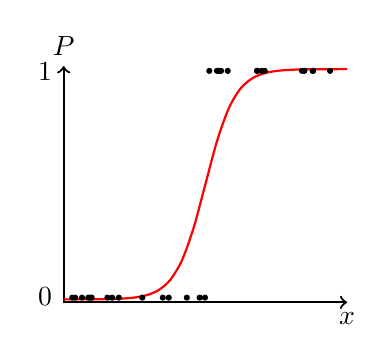
\begin{tikzpicture}[scale=0.15]
				% \draw [step=1, gray, very thin] (-12, -10) grid (12, 10);
				\draw [thick, <->] (-12, 10) node [anchor=south] {$P$} -- (-12, -10) -- (12, -10) node [anchor=north] {$x$};
				\draw [red, thick, smooth] plot [domain=-12:12] (\x, {(1 / (1 + exp(-0.8*\x)))*19.5 - 9.75});
				\draw plot [only marks, mark=*, mark size=6, domain=-8:8, samples=15] ({12.5*rnd - 0.5}, 9.6);
				\draw plot [only marks, mark=*, mark size=6, domain=-8:8, samples=15] ({-12.5*rnd + 0.5}, -9.6);
				\draw (-15, -9.5) node [anchor=west] {$0$};
				\draw (-15, 9.5) node [anchor=west] {$1$};
			\end{tikzpicture}
		\end{multicols}
		
		\columnbreak
		
		\section*{Definiciones estadísticas}
		
		Sean $\xi, \eta$ variables aleatorias, $a, b \in \mathbb{R}$ constantes, y $P$ denota probabilidad.
		
		\subsection*{Media}
		
		Definición: \quad $E(\xi) = \sum_{i=1}^{n}\xi_{i} \cdot P[\xi = \xi_{i}]$
		
		\begin{multicols}{2}
			Media poblacional:
			
			\begin{center}
				$\E(\xi) = \dfrac{1}{N}\sum_{i=1}^{N}\xi_{i}$
			\end{center}
			
			\columnbreak
			
			Media muestral:
			
			\begin{center}
				$\E(\xi) = \dfrac{1}{n}\sum_{i=1}^{n}\xi_{i}$
			\end{center}
		\end{multicols}
		
		Algunas propiedades:
		
		\begin{itemize}[leftmargin=*]
			\item $\E(a) = a$
			\item $\E(\xi + a) = \E(\xi) + a$
			\item $\E(a \cdot \xi) = a \cdot \E(\xi)$
			\item $\E(\xi \pm \eta) = \E(\xi) + \E(\eta)$
			\item $\E(\xi \cdot \eta) = \E(\xi) \cdot \E(\eta)$ \quad sólo si $\xi$ y $\eta$ son independientes.
			\item $\E(\xi - \E(\xi)) = 0$
			\item $\E(a \cdot \xi + b \cdot \eta) = a \cdot \E(\xi) + b \cdot \E(\eta)$
		\end{itemize}
		
		\subsection*{Varianza}
		
		Definición: \quad $\Var(\xi) = \E(\xi - \E(\xi))^{2}$
		
		\begin{multicols}{2}
			Varianza poblacional:
			
			\begin{center}
				$\Var(\xi) = \dfrac{\sum_{i=1}^{N} (\xi_{i} - \E(\xi))^2}{N}$
			\end{center}
			
			\columnbreak
			
			Varianza muestral:
			
			\begin{center}
				$\Var(\xi) = \dfrac{\sum_{i=1}^{n} (\xi_{i} - \E(\xi))^2}{n - 1}$
			\end{center}
		\end{multicols}
		
		Algunas propiedades:
		
		\begin{itemize}[leftmargin=*]
			\item $\Var(a) = 0$
			\item $\Var(\xi + a) = \Var(\xi)$
			\item $\Var(a \cdot \xi) = a^{2} \cdot \Var(\xi)$
			\item $\Var(\xi \pm \eta) = \Var(\xi) + \Var(\eta) \pm 2 \cdot \Cov(\xi, \eta)$
			\item $\Var(a \cdot \xi \pm b \cdot \eta) = a^{2} \cdot \Var(\xi) + b^{2} \cdot \Var(\eta) \pm 2 a b \cdot \Cov(\xi, \eta)$
		\end{itemize}
		
		\subsection*{Covarianza}
		
		Definición: \quad $\Cov(\xi, \eta) = \E[(\xi - E(\xi)) \cdot (\eta - E(\eta))]$
		
		\begin{multicols}{2}
			Covarianza poblacional:
			
			\begin{center}
				$\dfrac{\sum_{i=1}^{N} (\xi_{i} - \E(\xi)) \cdot (\eta_{i} - \E(\eta))}{N}$
			\end{center}
			
			\columnbreak
			
			Covarianza muestral:
			
			\begin{center}
				$\dfrac{\sum_{i=1}^{n} (\xi_{i} - \E(\xi)) \cdot (\eta_{i} - \E(\eta))}{n - 1}$
			\end{center}
		\end{multicols}
		
		Algunas propiedades:
		
		\begin{itemize}[leftmargin=*]
			\item $\Cov(\xi, a) = 0$
			\item $\Cov(\xi + a, \eta + b) = \Cov(\xi, \eta)$
			\item $\Cov(a \cdot \xi, b \cdot \eta) = a b \cdot \Cov(\xi, \eta)$
			\item $\Cov(\xi, \xi) = \Var(\xi)$
			\item $\Cov(\xi, \eta) = \Cov(\eta, \xi)$
		\end{itemize}
		
		\columnbreak
		
		\section*{Contraste de hipótesis (extra)}
		
		\begin{center}
			\begin{tabular}{ c | c | c }
				                 & $H_{0}$ verdadera       & $H_{0}$ falsa           \\ \hline
				Rechazar $H_{0}$ & Falso positivo          & Verdadero pos.          \\
				                 & Error Tipo I $(\alpha)$ & $(1 - \beta)$           \\ \hline
				Aceptar $H_{0}$  & Verdadero neg.          & Falso negativo          \\
				                 & $(1 - \alpha)$          & Error Tipo II $(\beta)$
			\end{tabular}
		\end{center}
		
		\columnbreak
		
		Típico contraste de una cola:
		
		\begin{center}
			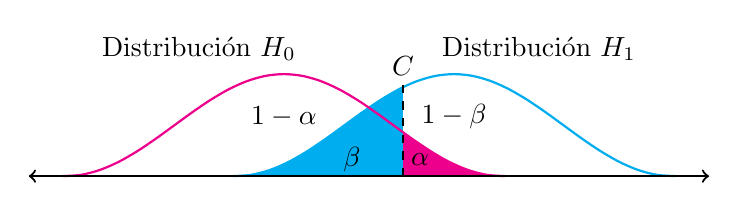
\begin{tikzpicture}[scale=0.108]
				\fill [magenta] (4, 0) -- plot [domain=4:16, smooth] (\x, {cos(\x*7 + 70)*6 + 6}); 
				\fill [cyan] (4, 0) -- plot [domain=-16:4, smooth] (\x, {cos(\x*7 - 70)*6 + 6}); 
				\draw [thick, cyan] plot [domain=-16:36, smooth] (\x, {cos(\x*7 - 70)*6 + 6}); 
				\draw [thick, magenta] plot [domain=-36:16, smooth] (\x, {cos(\x*7 + 70)*6 + 6}); 
				\draw [thick, <->] (-40, 0) -- (40, 0); 
				\draw [thick, dashed] (4, 0) -- (4, 11); 
				\node at (-20, 15) {Distribución $H_{0}$};
				\node at (20, 15) {Distribución $H_{1}$}; 
				\node at (-10, 7) {$1 - \alpha$}; 
				\node at (10, 7) {$1 - \beta$}; 
				\node at (6, 2) {$\alpha$}; 
				\node at (-2, 2) {$\beta$}; 
				\node at (4, 13) {$C$};
			\end{tikzpicture}
		\end{center}
		
		donde $(1 - \alpha)$ es nivel de confianza, $\alpha$ es nivel de significación, $C$ es valor crítico, $(1 - \beta)$ es potencia estadística.
		
		\section*{Bootstraping}
		
		\textbf{Problema} - Aprox. asint. a las distribuciones de los estadísticos de contraste no funcionan en muestras pequeñas.
		
		\textbf{Solución} - Boostrap es básicamente muestreo con reemplazo. Los datos observados se tratan como una población y se extraen varias muestras para recalcular un estimador o estadístico varias veces (mejora la precisión).
	\end{multicols}
	
	\begin{multicols}{2}
		\section*{VAR (Vector Autoregressive)}
		
		Un modelo VAR captura \textbf{interacciones dinámicas} entre series temporales. El VAR($p$):
		
		\begin{center}
			$y_{t} = A_{1} y_{t - 1}+ \cdots + A_{p} y_{t - p}+ B_{0} x_{t} + \cdots + B_{q} x_{t - q}+ CD_{t} + u_{t}$
		\end{center}
		
		donde:
		
		\begin{itemize}[leftmargin=*]
			\item $y_{t} = (y_{1t}, \ldots, y_{Kt})^{\tr}$ es un vector de $K$ series temporales observables endógenas.
			\item $A_{i}$'s son $K \times K$ matrices de coeficientes.
			\item $x_{t} = (x_{1t}, \ldots, x_{Mt})^{\tr}$ es un vector de $M$ series temporales observables exógenas.
			\item $B_{j}$'s son $K \times M$ matrices de coeficientes.
			\item $D_{t}$ es un vector que contiene todos los términos deterministas, que pueden ser: una constante, tendencia lineal, variables estacionales binarias, y/o cualquier otra variable ficticia especificada por el usuario.
			\item $C$ es una matriz de coeficientes de dimensión apropiada.
			\item $u_{t} = (u_{1t}, \ldots, u_{Kt})^{\tr}$ es un vector de $K$ series de ruido blanco.
		\end{itemize}
		
		El proceso es \textbf{estable} si:
		
		\begin{center}
			$\det(I_{K} - A_{1} z - \cdots - A_{p} z^{p}) \neq 0 \quad \mathrm{para}\quad \lvert z \rvert \leq 1$
		\end{center}
		
		\quad esto es, \textbf{no hay raíces} en y sobre el círculo unitario complejo.
		
		Por ejemplo, un modelo VAR con dos variables endógenas ($K = 2$), dos retardos ($p = 2$), una variable exógena contemporánea ($M = 1$), constante ($\mathrm{const}$) y tendencia ($\mathrm{Tend}_{t}$):
		
		\begin{center}
			\scalebox{0.80}{
				$
				\begin{bmatrix}
					y_{1t} \\
					y_{2t}
				\end{bmatrix}
				=
				\begin{bmatrix}
					a_{11, 1} & a_{12, 1} \\
					a_{21, 1} & a_{22, 1}
				\end{bmatrix}
				\cdot
				\begin{bmatrix}
					y_{1, t - 1} \\
					y_{2, t - 1}
				\end{bmatrix}
				+
				\begin{bmatrix}
					a_{11, 2} & a_{12, 2} \\
					a_{21, 2} & a_{22, 2}
				\end{bmatrix}
				\cdot
				\begin{bmatrix}
					y_{1, t - 2} \\
					y_{2, t - 2}
				\end{bmatrix}
				+
				\begin{bmatrix}
					b_{11} \\
					b_{21}
				\end{bmatrix}
				\cdot
				\begin{bmatrix}
					x_{t}
				\end{bmatrix}
				+
				\begin{bmatrix}
					c_{11} & c_{12} \\
					c_{21} & c_{22}
				\end{bmatrix}
				\cdot
				\begin{bmatrix}
					\mathrm{const}    \\
					\mathrm{Tend}_{t}
				\end{bmatrix}
				+
				\begin{bmatrix}
					u_{1t} \\
					u_{2t}
				\end{bmatrix}
				$
			}
		\end{center}
		
		Visualizando las ecuaciones por separado:
		
		\begin{center}
			$y_{1t} = a_{11, 1} y_{1, t - 1} + a_{12, 1} y_{2, t - 1} + a_{11, 2} y_{1, t - 2} + a_{12, 2} y_{2, t - 2} + b_{11} x_{t} + c_{11} + c_{12} \mathrm{Tend}_{t} + u_{1t}$
			
			$y_{2t} = a_{21, 1} y_{2, t - 1} + a_{22, 1} y_{1, t - 1} + a_{21, 2} y_{2, t - 2} + a_{22, 2} y_{1, t - 2} + b_{21} x_{t} + c_{21} + c_{22} \mathrm{Tend}_{t} + u_{2t}$
		\end{center}
		
		Si hay una raíz unitaria, el determinante es cero para $z = 1$, entonces una o todas las variables son integrados y el modelo VAR ya no es apropiado (es inestable).
		
		\columnbreak
		
		\section*{VECM (Vector Error Correction Model)}
		
		Si existen \textbf{relaciones cointegradoras} en un sistema de variables, la forma VAR no es la más conveniente. Es mejor usar un VECM, esto es, el VAR en niveles sustrayendo $y_{t - 1}$ de ambos lados. El VECM($p - 1$):
		
		\begin{center}
			$\Delta y_{t} = \Pi y_{t - 1} + \Gamma_{1} \Delta y_{t - 1} + \cdots + \Gamma_{p - 1} \Delta y_{t - p + 1} + B_{0} x_{t} + \cdots + B_{q} x_{t - q} + CD_{t} + u_{t}$
		\end{center}
		
		donde:
		
		\begin{itemize}[leftmargin=*]
			\item $y_{t}$, $x_{t}$, $D_{t}$ y $u_{t}$ son como especificados en VAR.
			\item $\Pi = - (I_{K} - A_{1} - \cdots - A_{p})$ para $i = 1, \ldots, p - 1$; $\Pi y_{t - 1}$ es referido como la parte a \textbf{largo plazo}.
			\item $\Gamma_{i} = - (A_{i + 1} + \cdots + A_{p})$ para $i = 1, \ldots, p - 1$ es referido como parámetros a \textbf{corto plazo}.
			\item $A_{i}$, $B_{j}$ y $C$ son matrices de coeficientes de dimensiones apropiadas.
		\end{itemize}
		
		Si el proceso VAR($p$) es inestable (no hay raíces), $\Pi$ puede ser escrito como el producto de ($K \times r$) matrices $\alpha$ (\textbf{matriz de carga}) y $\beta$ (\textbf{matriz de cointegración}) con $\rk(\Pi) = \rk(\alpha) = \rk(\beta) = r$ (\textbf{rango cointegrador}) como $\Pi = \alpha \beta^{\tr}$.
		
		\begin{itemize}[leftmargin=*]
			\item $\beta^{\tr} y_{t - 1}$ contiene las relaciones cointegradoras.
		\end{itemize}
		
		Por ejemplo, si hay tres variables endógenas ($K = 3$) con dos relaciones cointegradoras ($r = 2$), la parte a largo plazo del VECM:
		
		\begin{center}
			\scalebox{0.95}{
				$\Pi y_{t - 1} = \alpha \beta^{\tr} y_{t - 1} =
				\begin{bmatrix}
					\alpha_{11} & \alpha_{12} \\
					\alpha_{21} & \alpha_{22} \\
					\alpha_{31} & \alpha_{32}
				\end{bmatrix}
				\begin{bmatrix}
					\beta_{11} & \beta_{21} & \beta_{31} \\
					\beta_{12} & \beta_{22} & \beta_{32}
				\end{bmatrix}
				\begin{bmatrix}
					y_{1, t - 1} \\
					y_{2, t - 1} \\
					y_{3, t - 1}
				\end{bmatrix}
				=
				\begin{bmatrix}
					\alpha_{11} ec_{1, t - 1} + \alpha_{12} ec_{2, t - 1} \\
					\alpha_{21} ec_{1, t - 1} + \alpha_{22} ec_{2, t - 1} \\
					\alpha_{31} ec_{1, t - 1} + \alpha_{32} ec_{2, t - 1}
				\end{bmatrix}
				$
			}
		\end{center}
		
		\quad donde:
		
		\begin{center}
			$ec_{1, t - 1} = \beta_{11} y_{1, t - 1} + \beta_{21} y_{2, t - 1} + \beta_{31} y_{3, t - 1}$
			
			$ec_{2, t - 1} = \beta_{12} y_{1, t - 1} + \beta_{22} y_{2, t - 1} + \beta_{32} y_{3, t - 1}$
		\end{center}
	\end{multicols}
\end{document}